\documentclass{beamer}

% Indicate to use hyperlink and in which color put them 
\usepackage{hyperref}
\hypersetup{
    colorlinks=true,
    linkcolor=orange,
    filecolor=magenta,      
    urlcolor=pink,
}

% Define the presentation them
\usetheme{Warsaw}

% Set the general color
\definecolor{Dark-lavender}{rgb}{0.45, 0.31, 0.59}
\usecolortheme[named=Dark-lavender]{structure}

\usepackage{hyperref}

\author{Damien Ribeiro}
\institute{
\includegraphics[height=0.8cm]{../images/tinkou.pdf}}

\title{Cloud \& Devops}
\subtitle{Introduction for business actors}

\begin{document}
	\frame {
		\titlepage
	}
	
		
	\frame{
		\frametitle{Outline}
		\tableofcontents[hideallsubsections]
	}

	\section{Devops}
	\subsection{DevOps}
	\begin{frame}
		\frametitle{Definition}
		"\textit{A set of practices intended to reduce the time between committing a change to a system and the change being placed into normal production, while ensuring high quality.}"
		
		\begin{flushright}
			{\footnotesize [Len Bass, Ingo Weber, and Liming Zhu \newline from the CSIRO and the Software Engineering Institute]}
		\end{flushright}
	\end{frame}
	
	\begin{frame}
		\frametitle{Definition}
		\textit{A set of practices to reconcile Dev and Ops.}
	\end{frame}

	\begin{frame}
		\frametitle{Definition}
		\textit{An extension of Agility to include Ops}
	\end{frame}
	
	\subsection{Objectives}
	\begin{frame}
		\frametitle{Objectives}
		
		\begin{itemize}
			\item Increase release rate
			\item Decrease Time to Market
			\item Decrease production delivery's failures
			\item Decrease failure effects
		\end{itemize}
	\end{frame}
	
	\subsection{Practices}
	\begin{frame}
		\frametitle{Practices}

		\begin{itemize}		
			\item Communicate \& share information
			\item Be responsible \& autonomous
			\item Test \& ensure product quality
			\item \textit{Done it, Run it}
			\item Automation
			\item Non-event
		\end{itemize}
	\end{frame}
	
	\section{Microservices}
	
	\subsection{An example}
	\begin{frame}
		\frametitle{An example}
		Better an example than a \href{https://en.wikipedia.org/wiki/Microservices}{definition}.
	\end{frame}
	
	\begin{frame}
		\frametitle{An example}
		\center{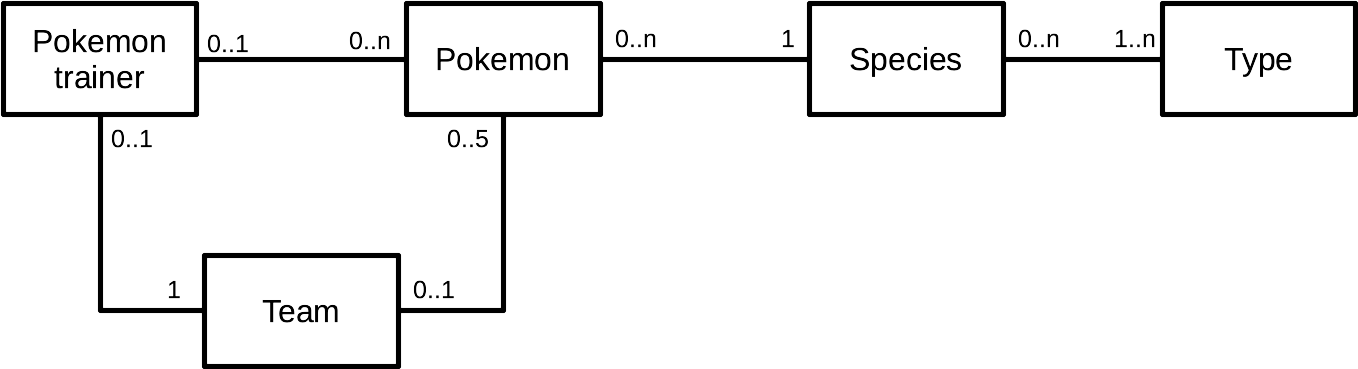
\includegraphics[width=10cm]{images/microservices-1.png}}
	\end{frame}

	\begin{frame}
		\frametitle{An example}
		\center{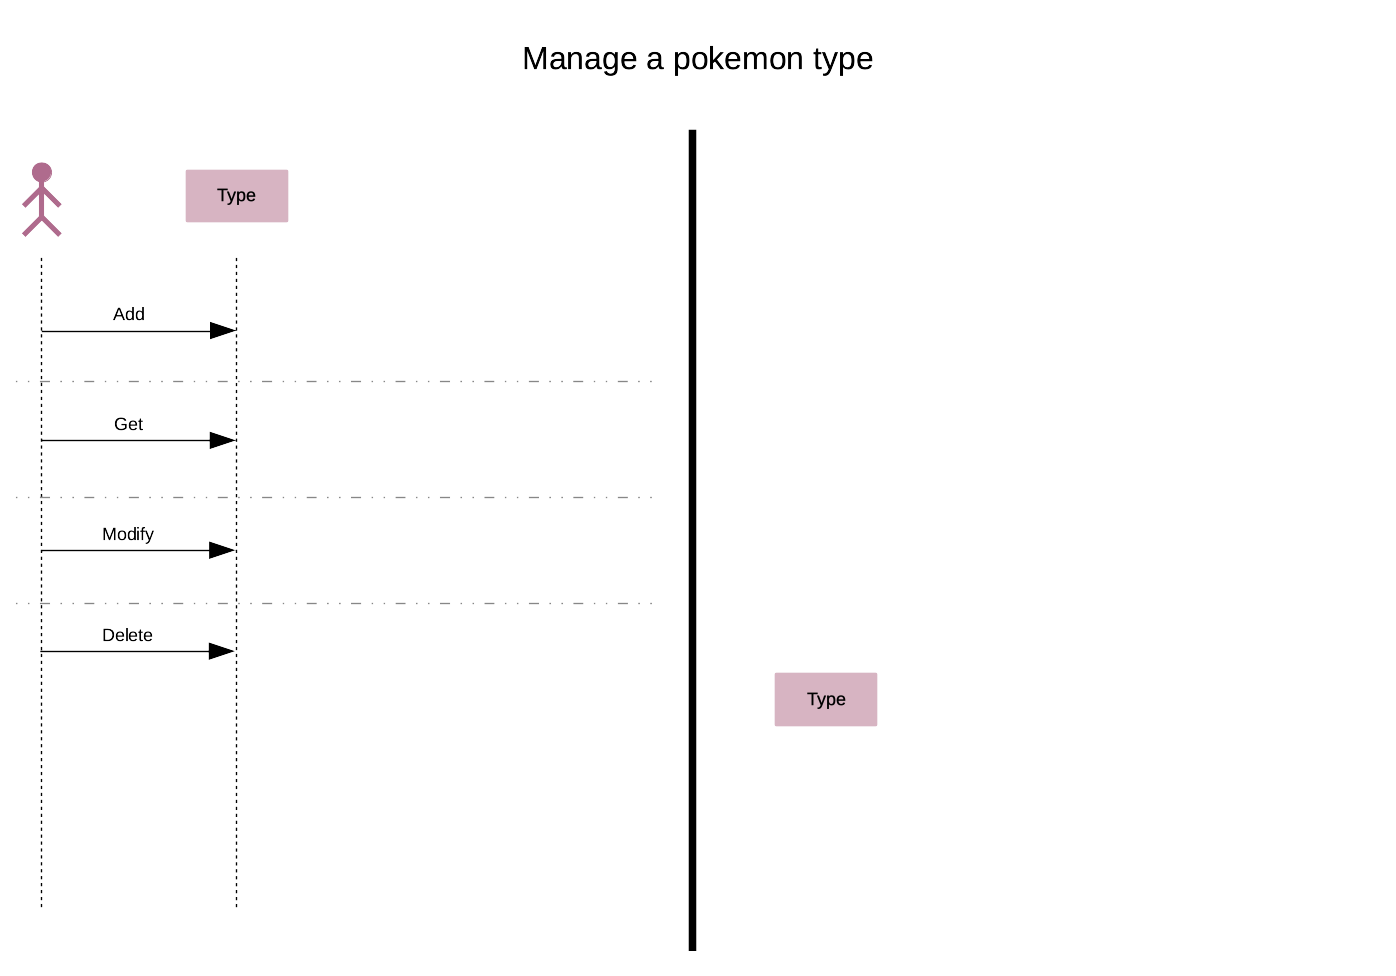
\includegraphics[height=6.5cm]{images/microservices-2.png}}
	\end{frame}

	\begin{frame}
		\frametitle{An example}
		\center{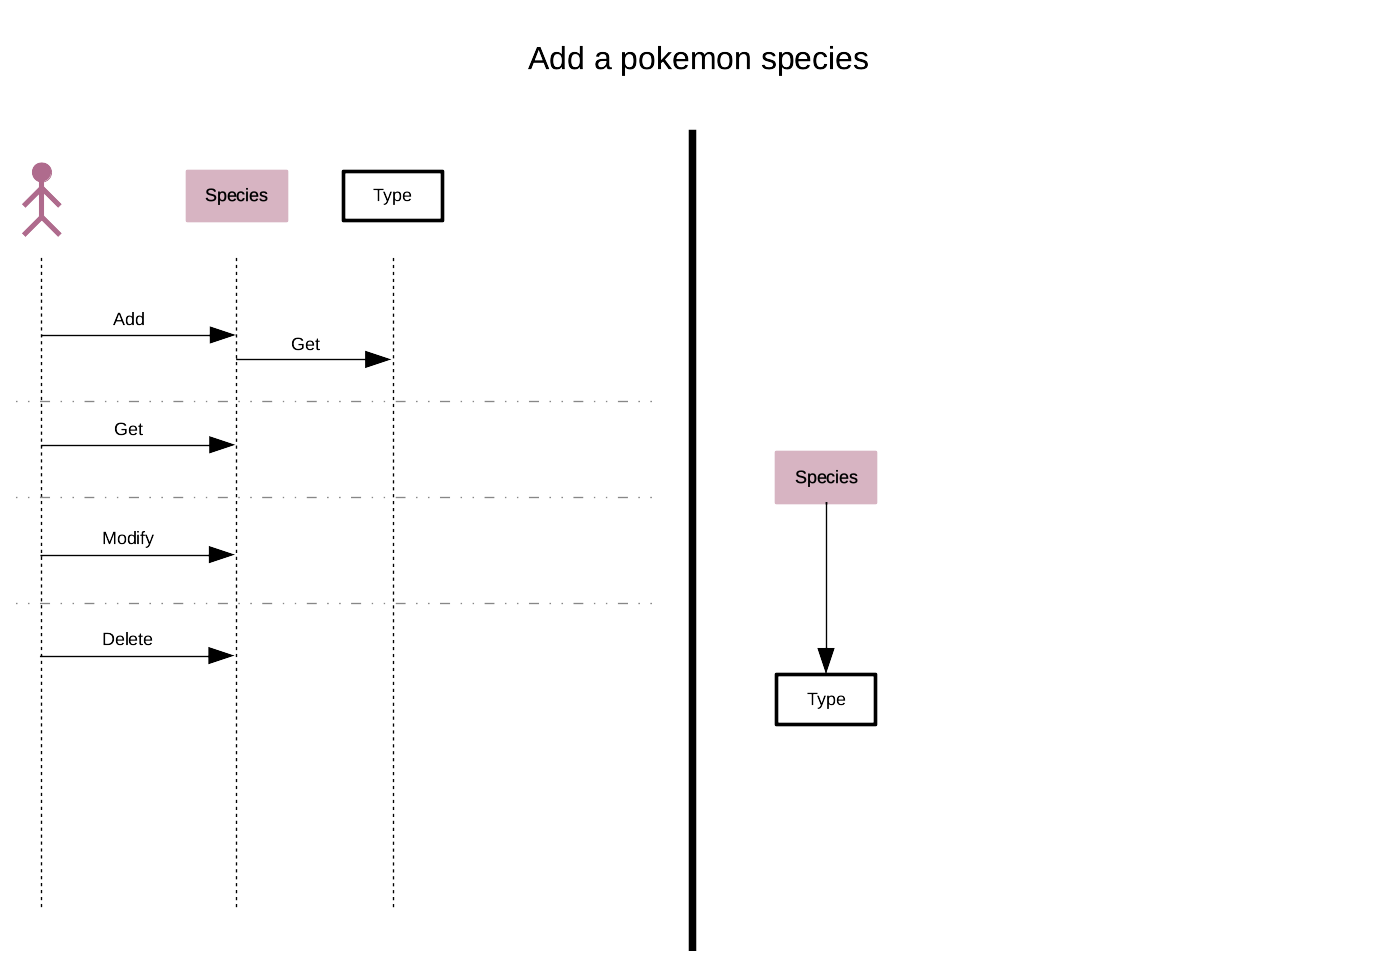
\includegraphics[height=6.5cm]{images/microservices-3.png}}
	\end{frame}

	\begin{frame}
		\frametitle{An example}
		\center{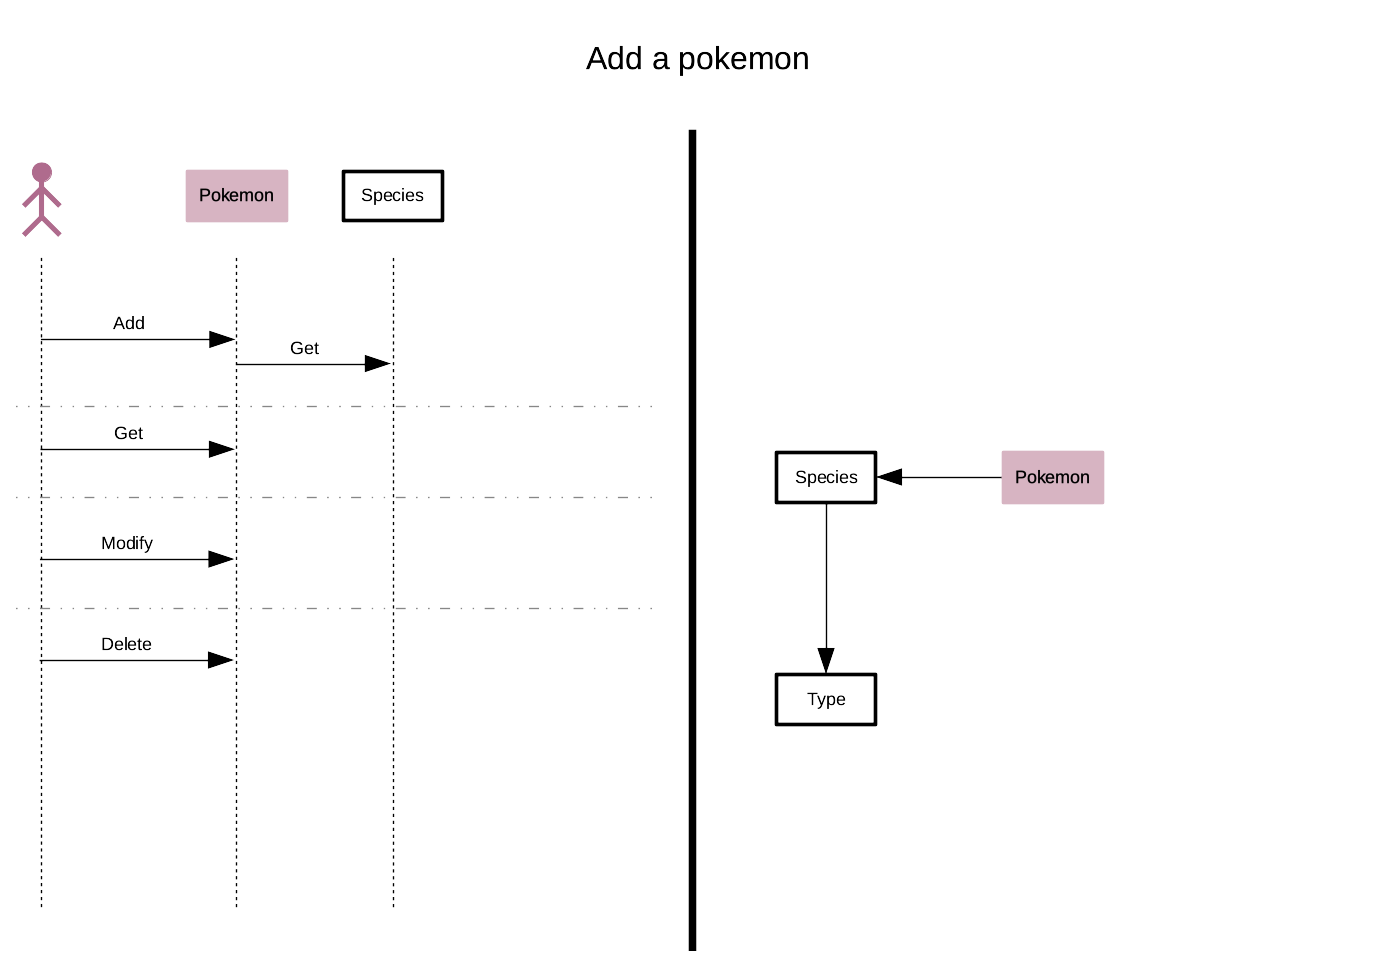
\includegraphics[height=6.5cm]{images/microservices-4.png}}
	\end{frame}

	\begin{frame}
		\frametitle{An example}
		\center{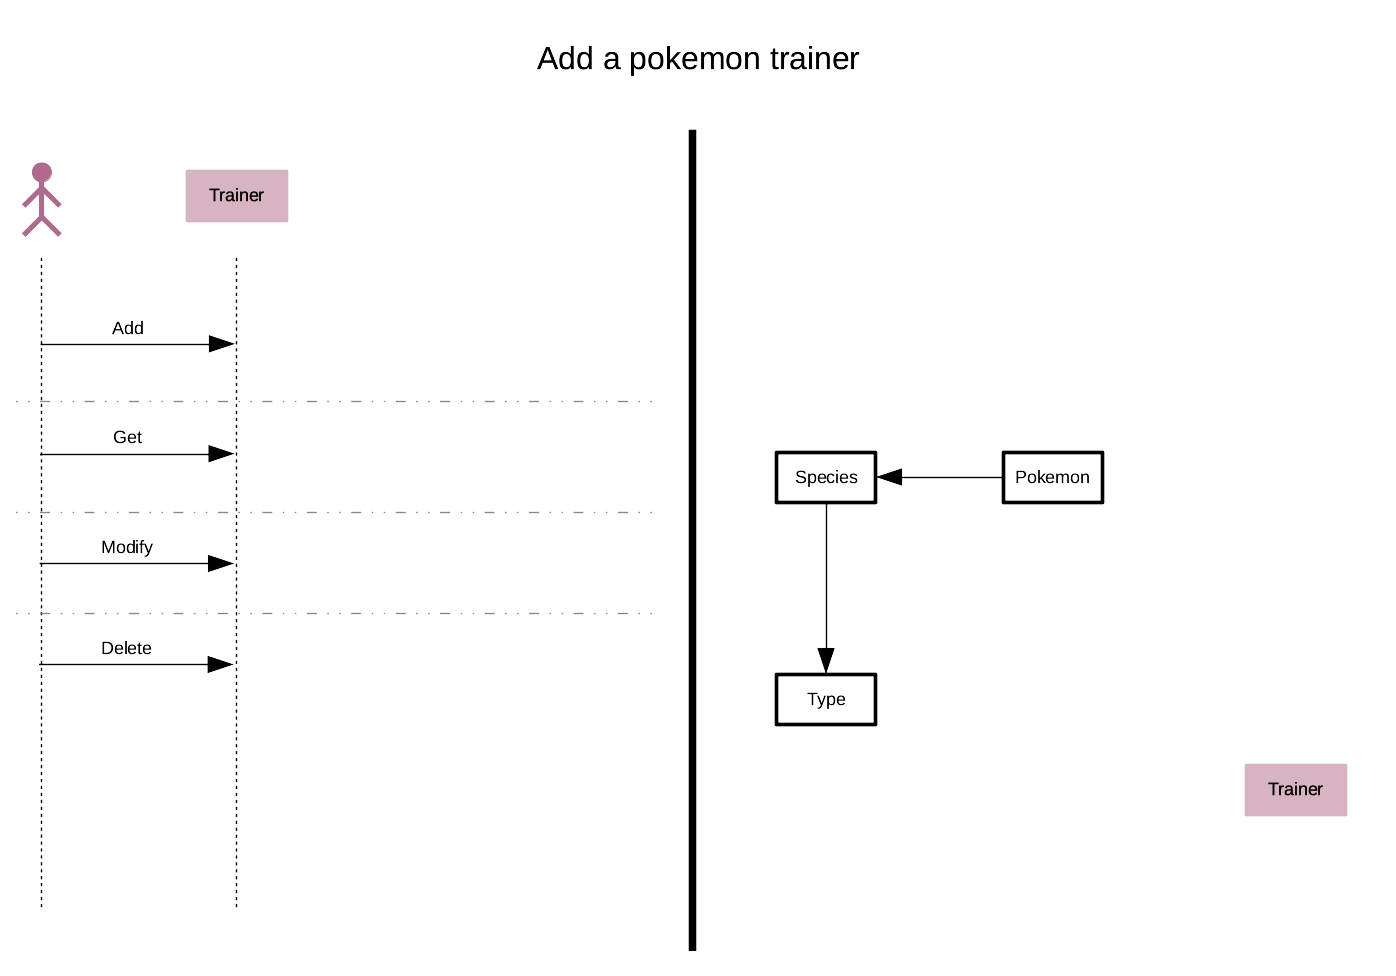
\includegraphics[height=6.5cm]{images/microservices-5.png}}
	\end{frame}

	\begin{frame}
		\frametitle{An example}
		\center{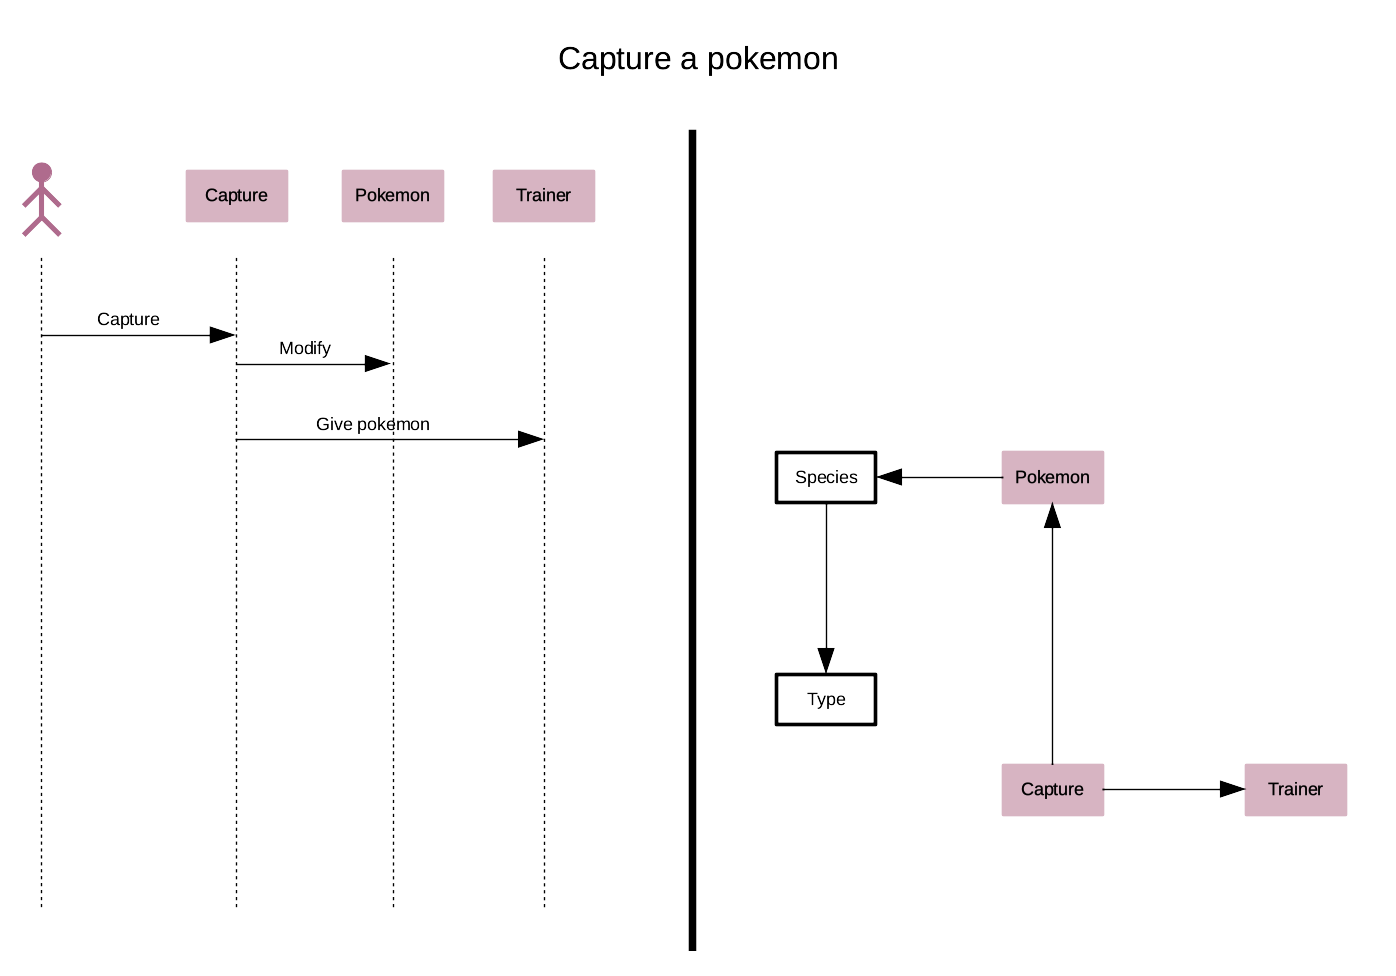
\includegraphics[height=6.5cm]{images/microservices-6.png}}
	\end{frame}

	\begin{frame}
		\frametitle{An example}
		\center{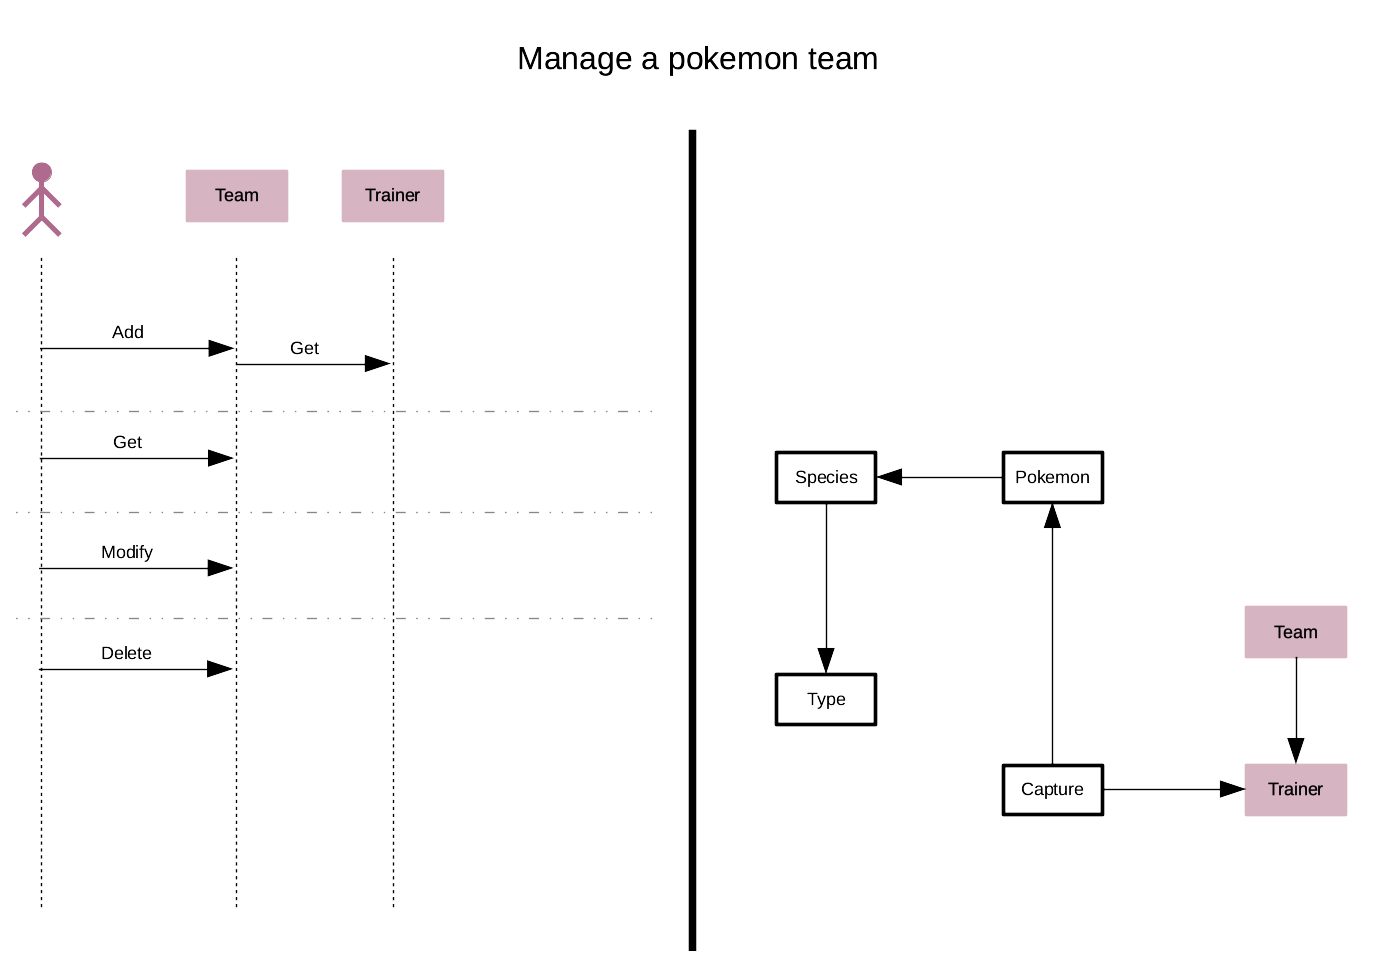
\includegraphics[height=6.5cm]{images/microservices-7.png}}
	\end{frame}

	\begin{frame}
		\frametitle{An example}
		\center{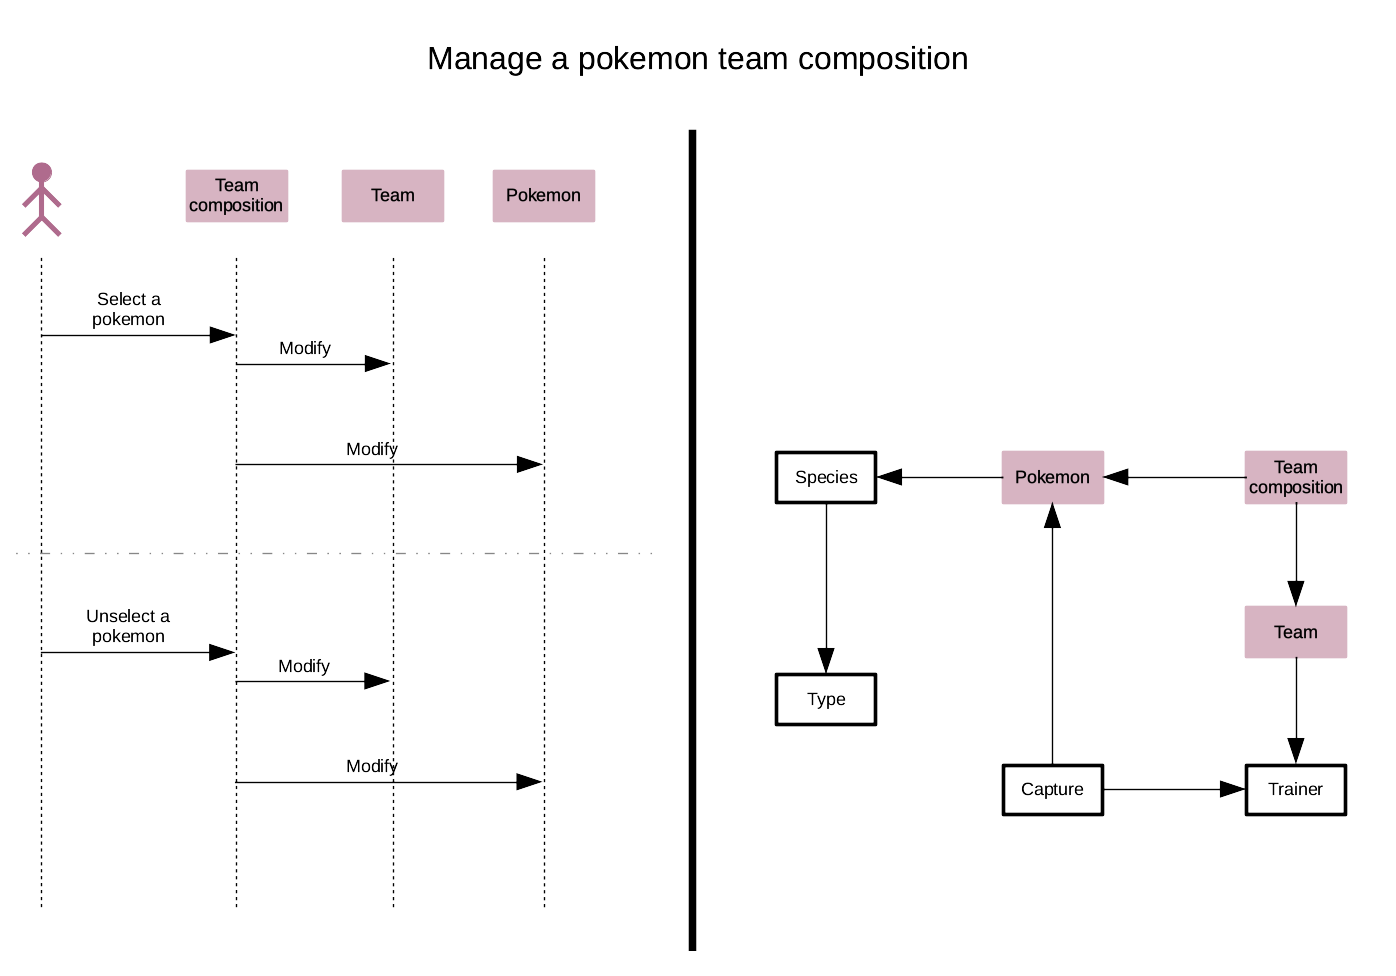
\includegraphics[height=6.5cm]{images/microservices-8.png}}
	\end{frame}

	\begin{frame}
		\frametitle{An example}
		\center{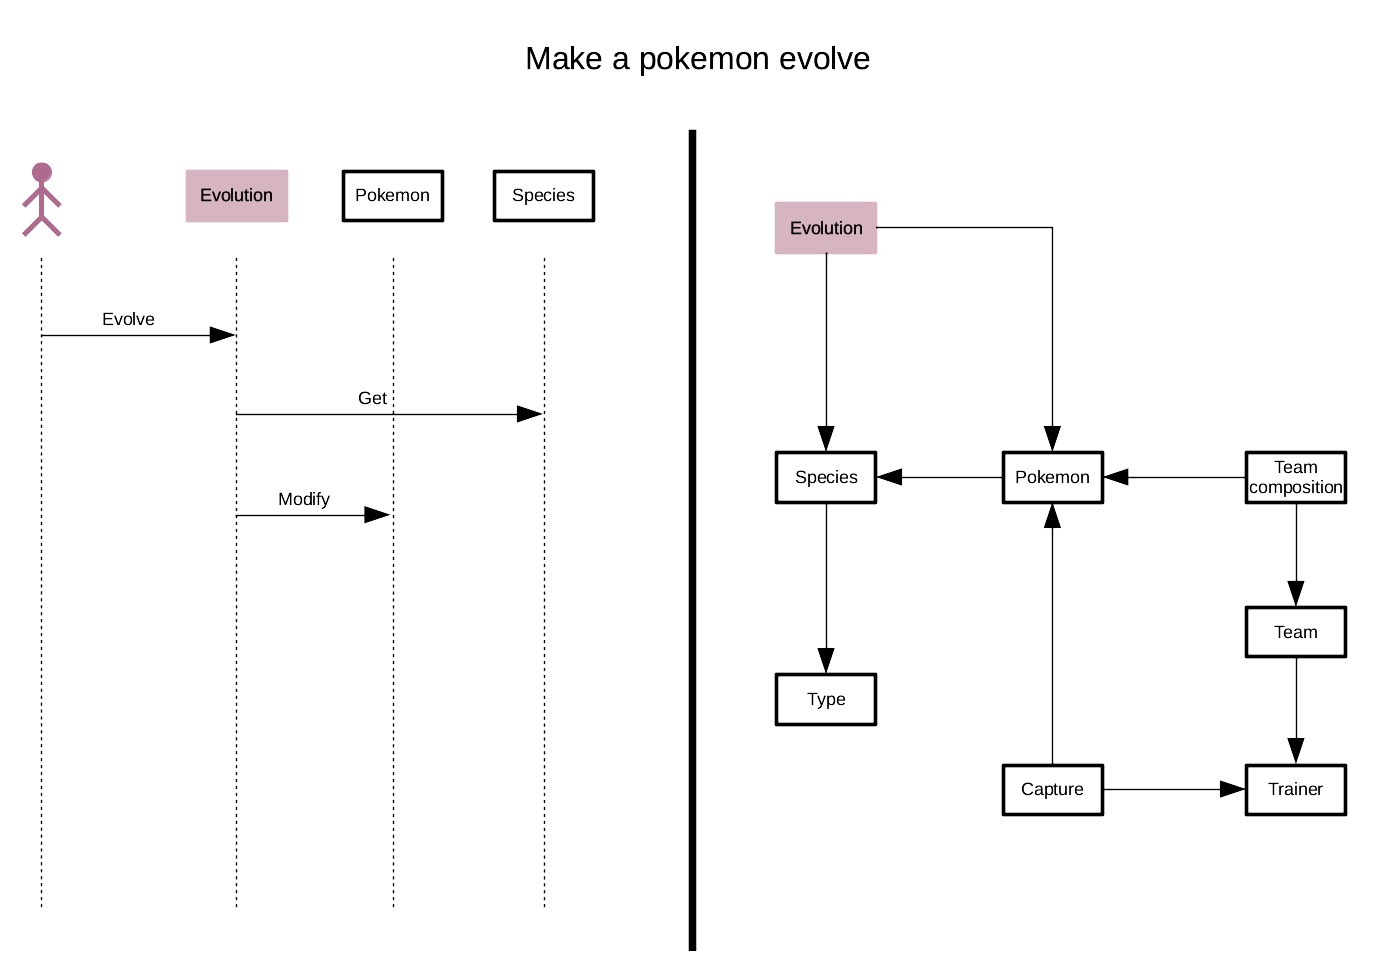
\includegraphics[height=6.5cm]{images/microservices-9.png}}
	\end{frame}
	
	\subsection{Requirements}
	\begin{frame}
		\frametitle{Requirements}
		
		\begin{itemize}
			\item User stories aligned with components
			\medskip
			\item Minimize the number of components impacted
			\medskip
			\item Minimize the scope of each user story
		\end{itemize}
	\end{frame}
	
	\section{Cloud}
	\subsection{Cloud definition}
	\begin{frame}
		\frametitle{Cloud definition}
		
		\pause 
		
		\begin{block}{\href{https://en.wikipedia.org/wiki/Cloud_computing}{Definition}}
			\begin{itemize}
				\item On-demand availability of computer system resources
				\item Coherence
				\item Economies of scale
			\end{itemize}
		\end{block}

		\pause		
		
		\begin{block}{Some features}
			\begin{itemize}
				\item Device and location independence
				\item Flexibility
				\item Scalability
				\item Reliability
			\end{itemize}
		\end{block}
	\end{frame}		
	
	\subsection{Container \& scheduling}
	\begin{frame}
		\frametitle{What is a container?}
		\center{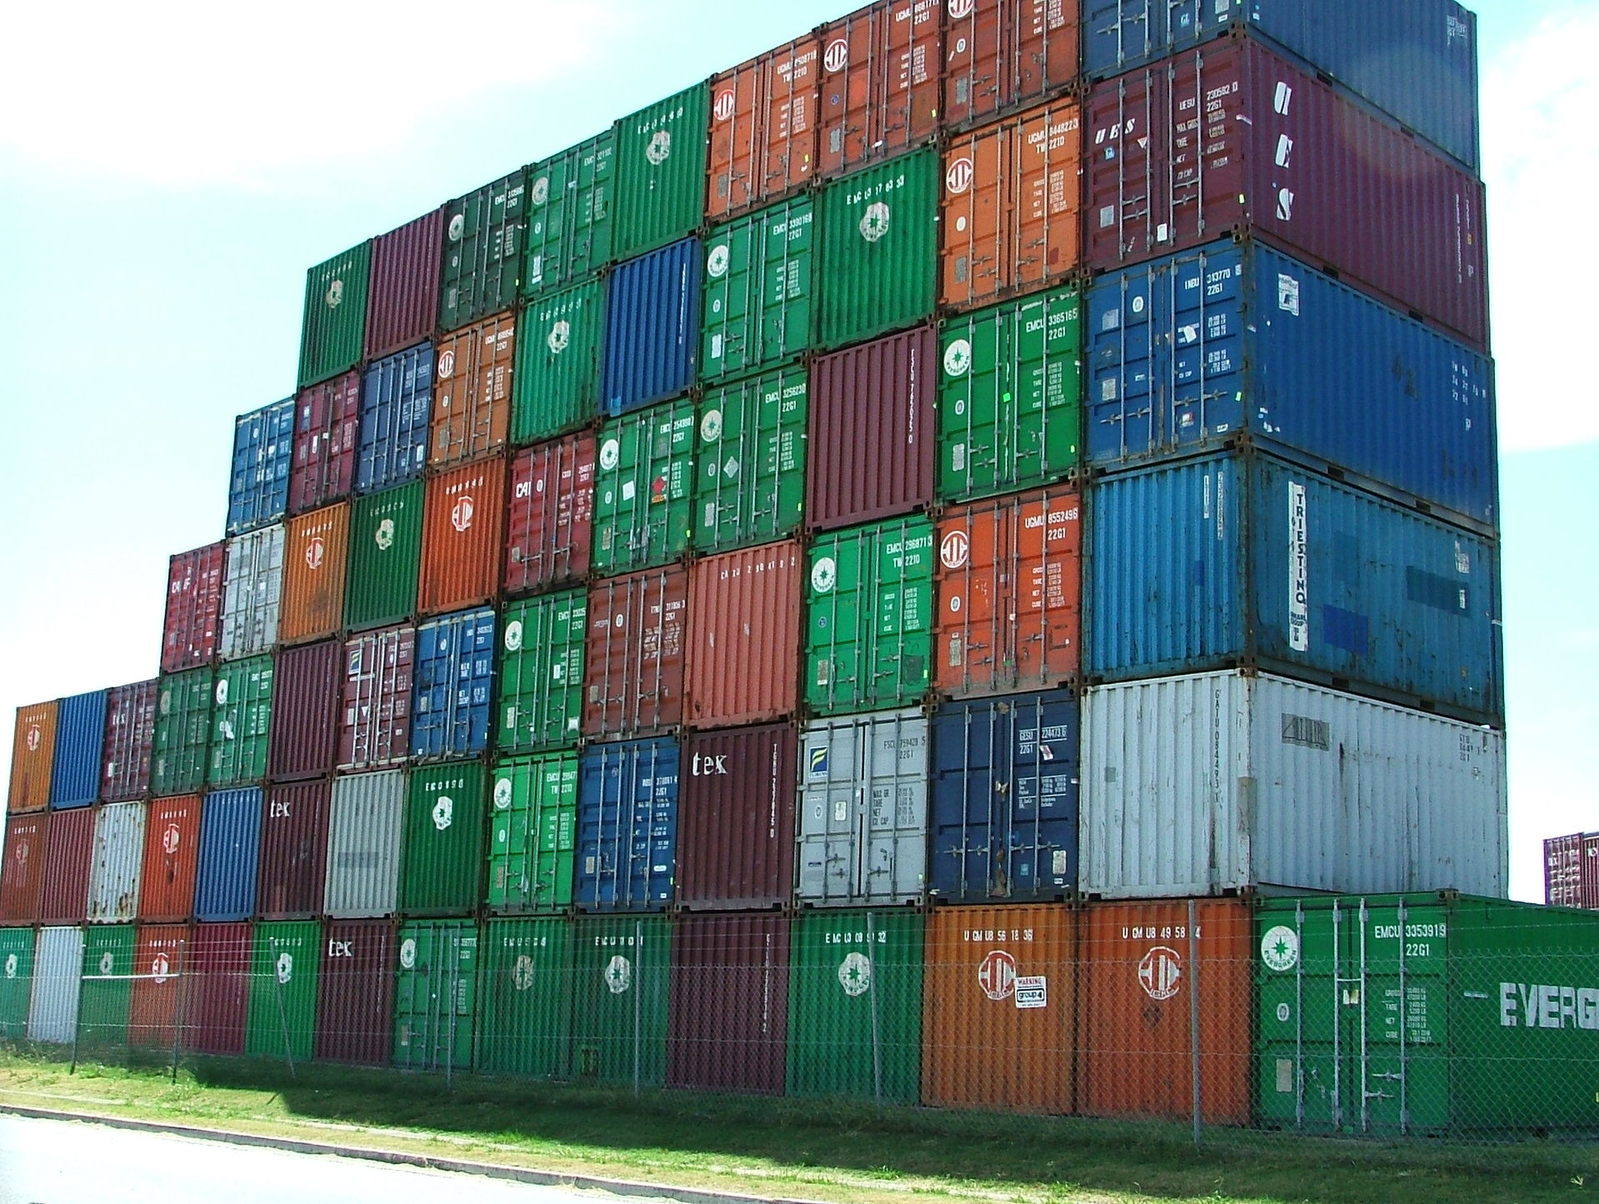
\includegraphics[height=6cm]{images/containers.jpg}}
	\end{frame}
	
	\begin{frame}
		\frametitle{A cluster architecture}
		\center{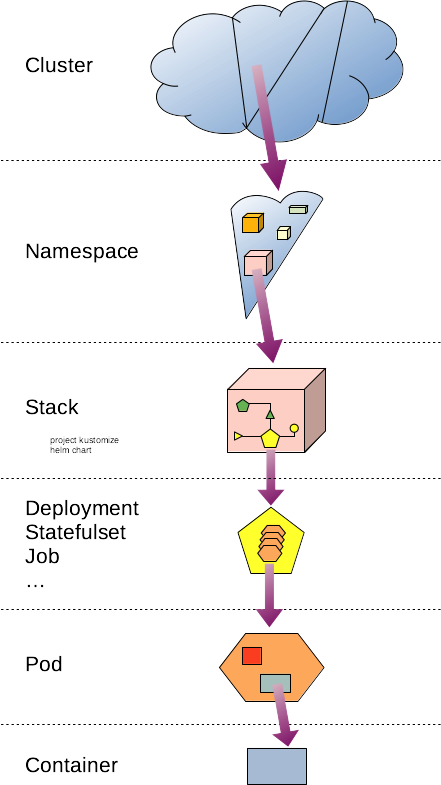
\includegraphics[height=6.5cm]{images/fromCluster2container.png}}
	\end{frame}
	
	\begin{frame}
		\frametitle{Scheduling example}
		\center{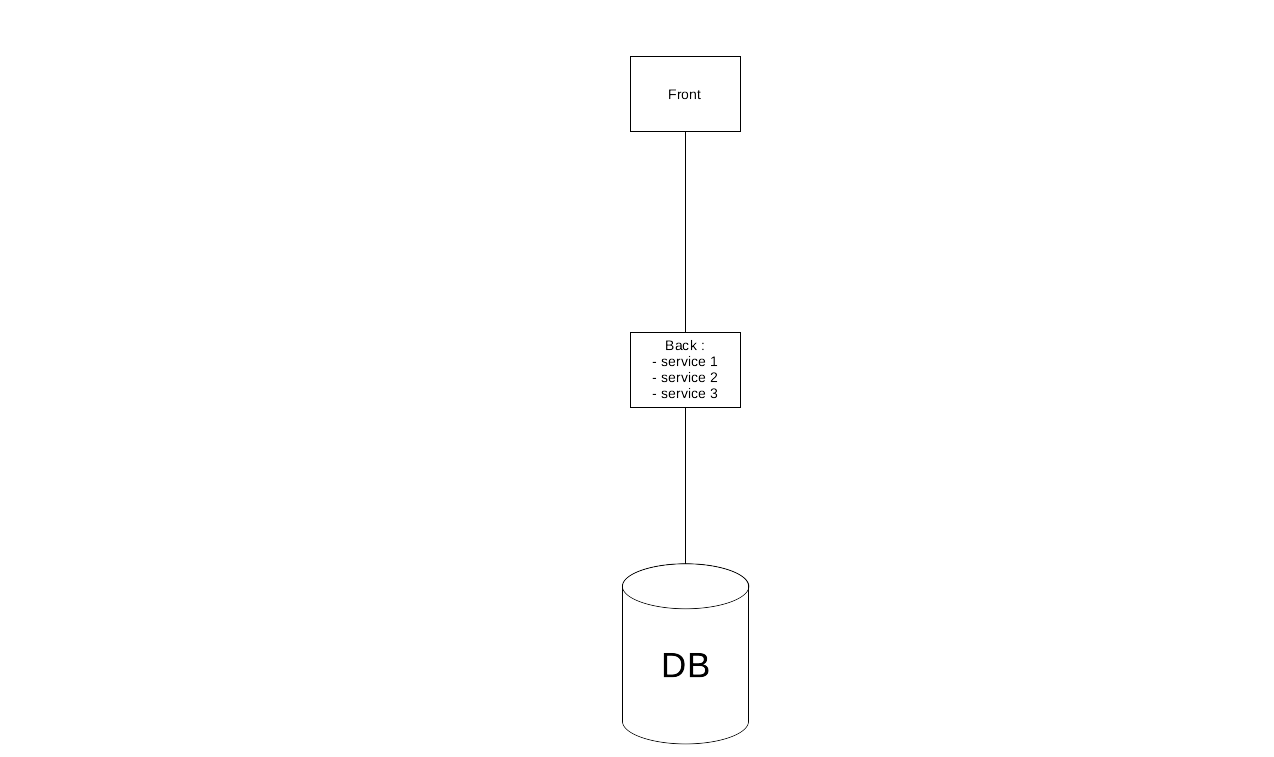
\includegraphics[height=6cm]{images/scalingExample-1.png}}
	\end{frame}

	\begin{frame}
		\frametitle{Scheduling example}
		\center{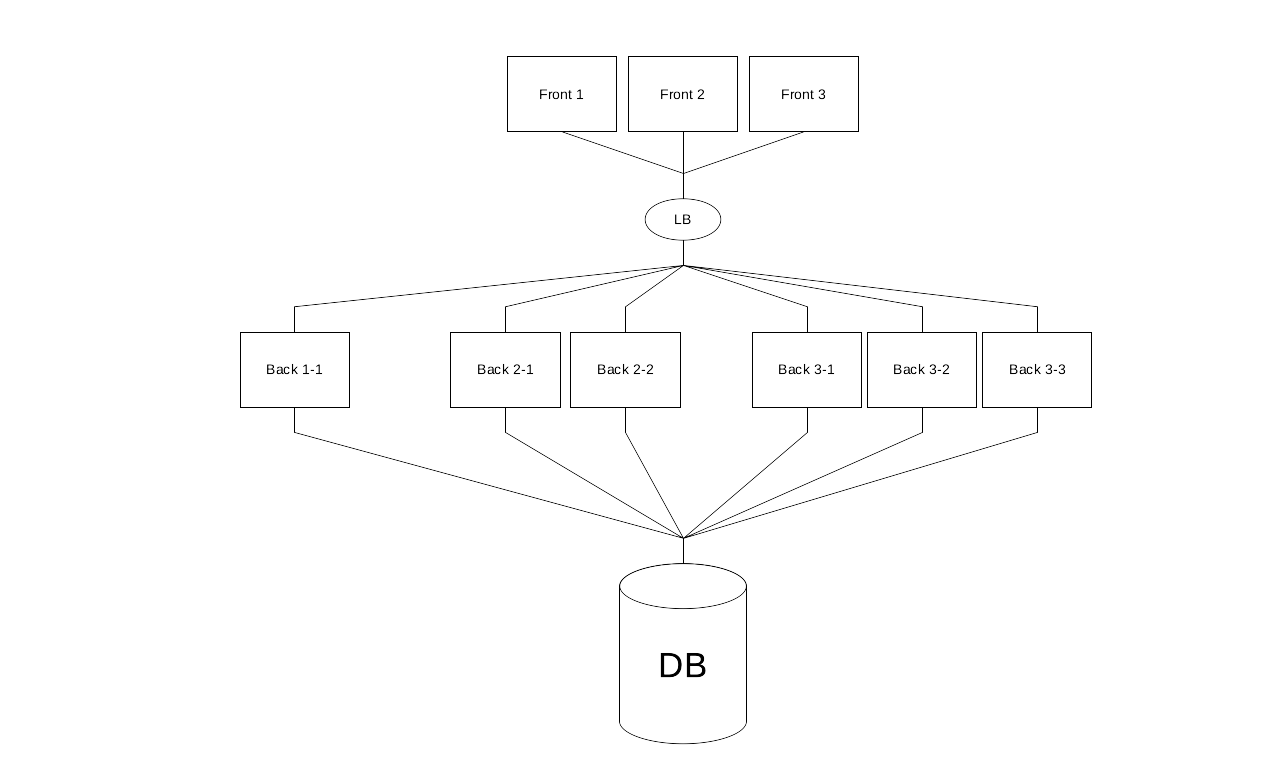
\includegraphics[height=6cm]{images/scalingExample-2.png}}
	\end{frame}

	\begin{frame}
		\frametitle{Scheduling example}
		\center{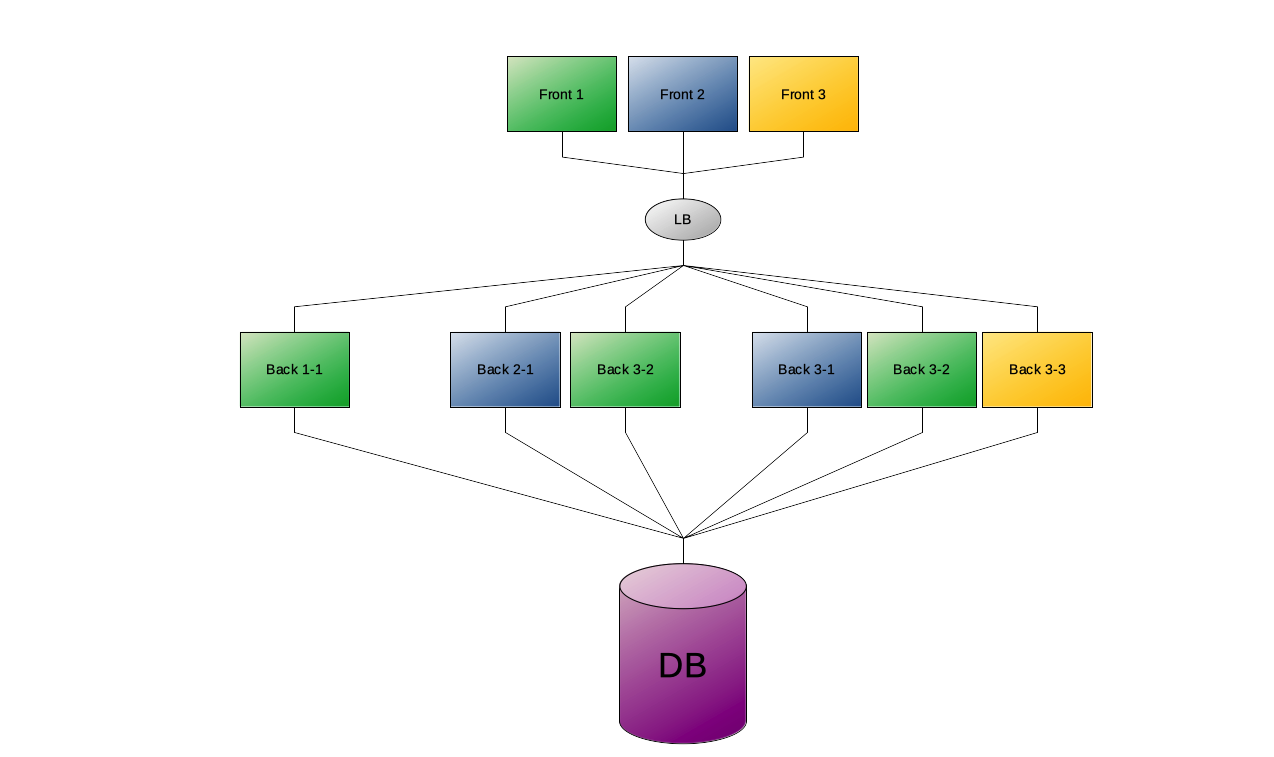
\includegraphics[height=6cm]{images/scalingExample-3.png}}
	\end{frame}

	\begin{frame}
		\frametitle{Scheduling example}
		\center{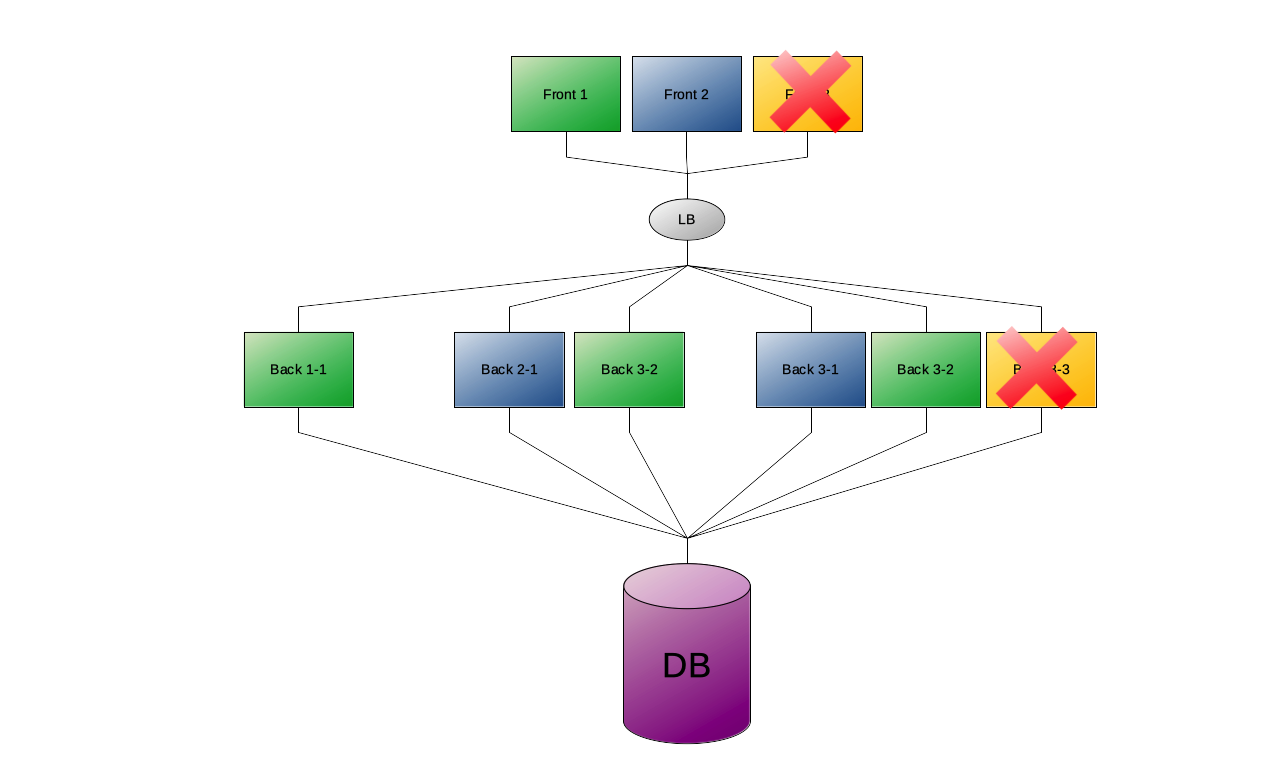
\includegraphics[height=6cm]{images/scalingExample-4.png}}
	\end{frame}

	\begin{frame}
		\frametitle{Scheduling example}
		\center{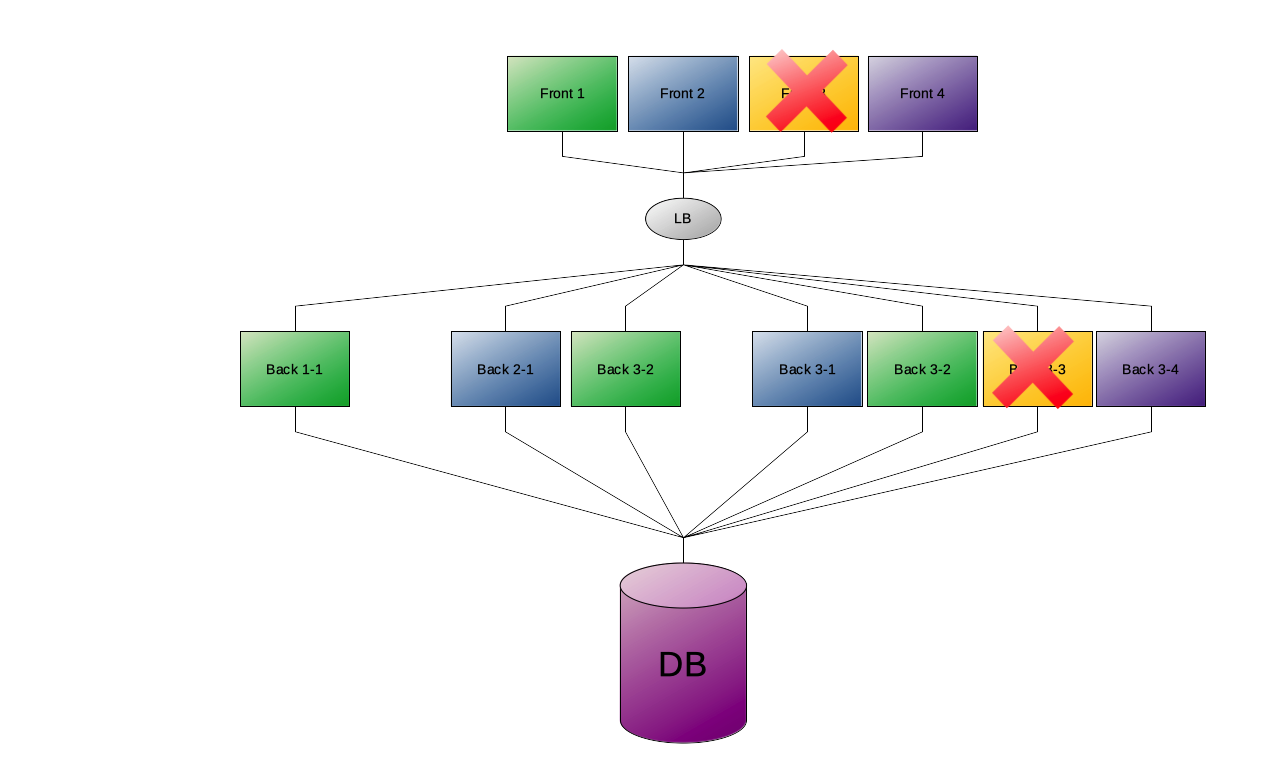
\includegraphics[height=6cm]{images/scalingExample-5.png}}
	\end{frame}

	\begin{frame}
		\frametitle{Scheduling example}
		\center{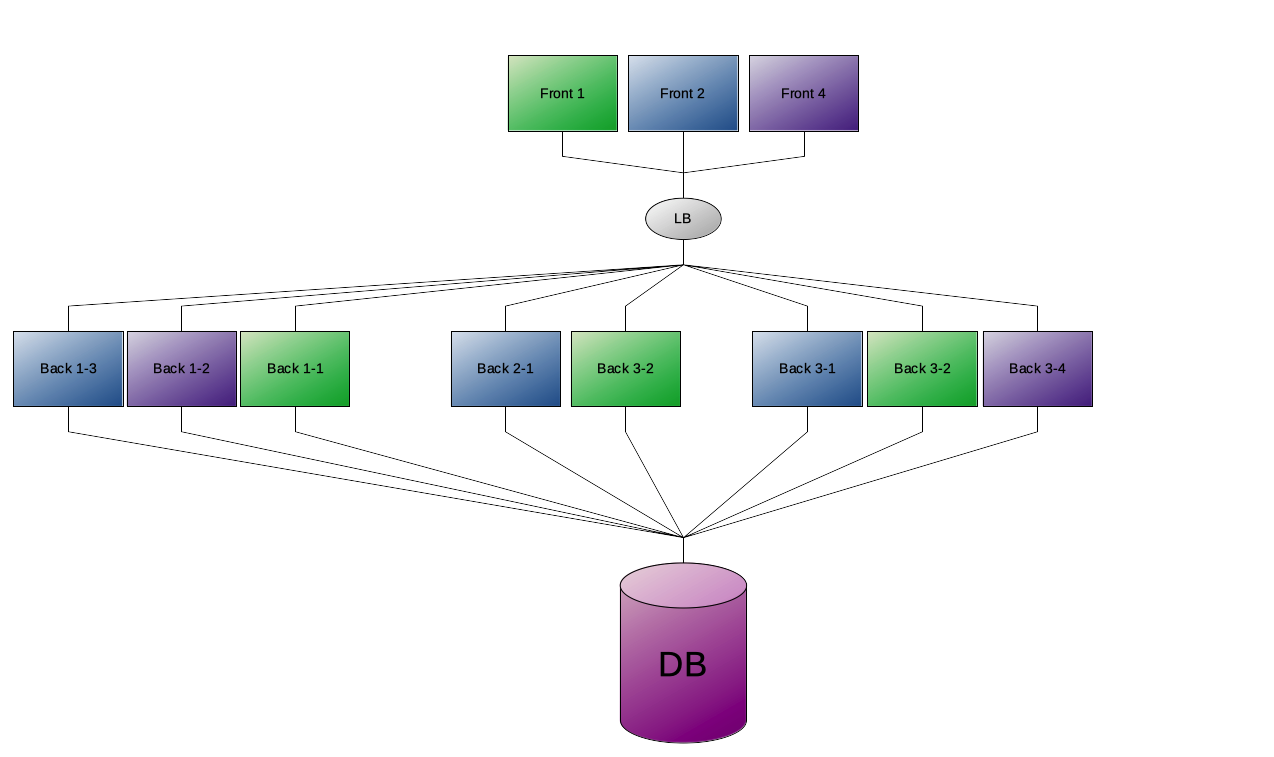
\includegraphics[height=6cm]{images/scalingExample-6.png}}
	\end{frame}

	\begin{frame}
		\frametitle{Scheduling example}
		\center{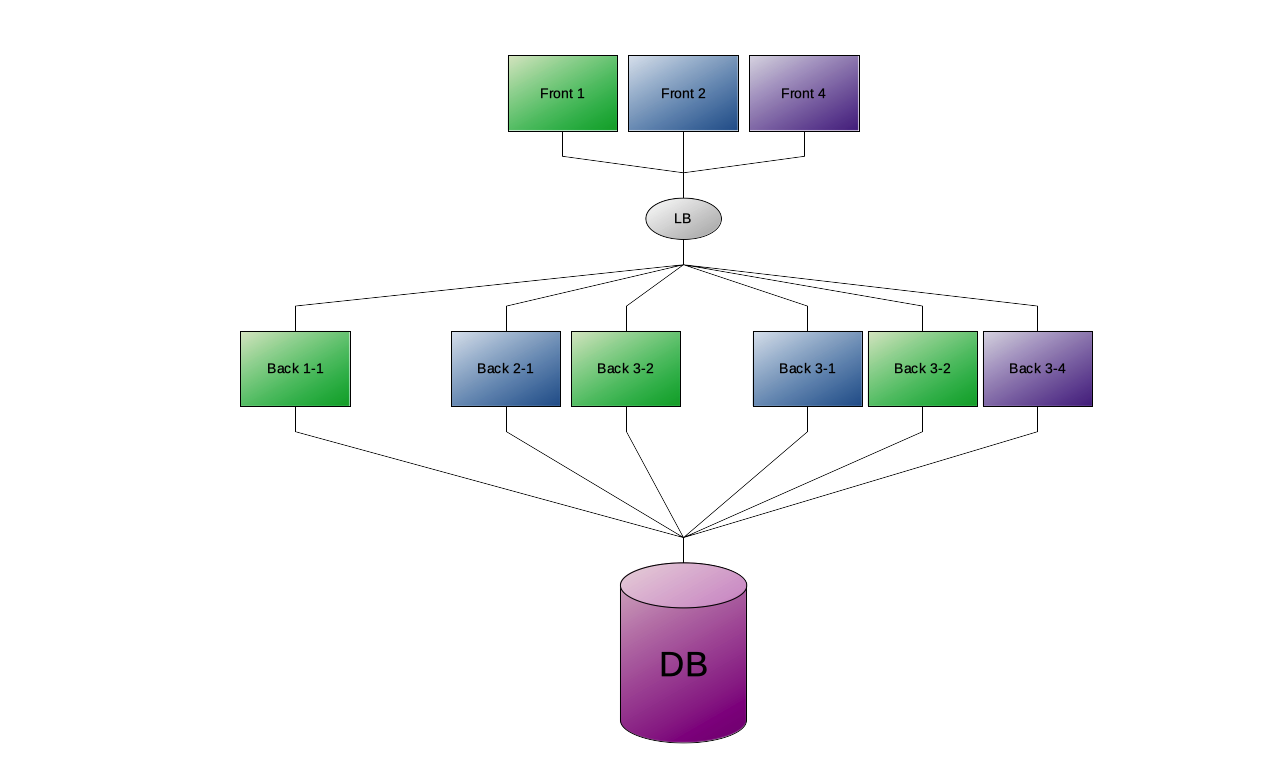
\includegraphics[height=6cm]{images/scalingExample-7.png}}
	\end{frame}
		
	\subsection{Requirements \& acceptance tests}
	\begin{frame}
		\frametitle{Concurrency}
		\center{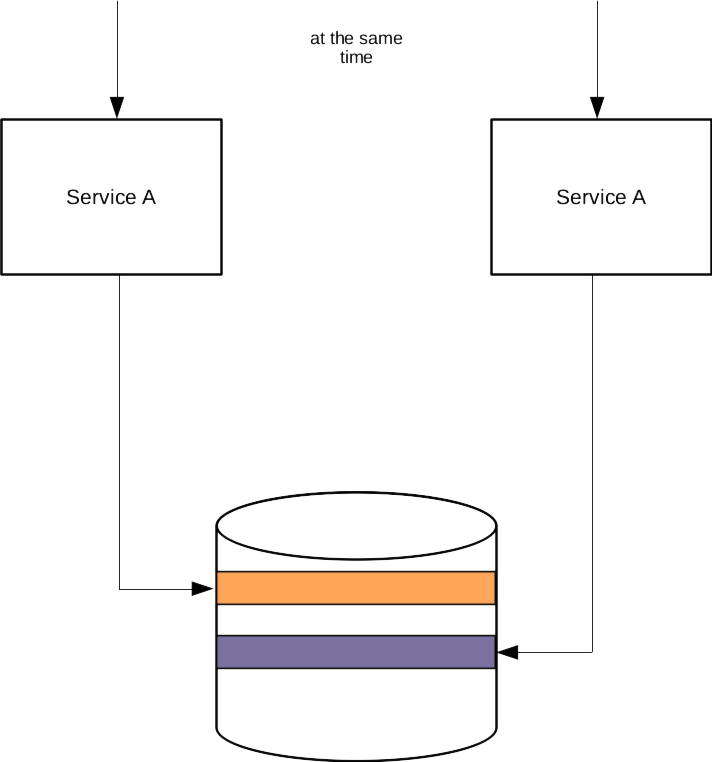
\includegraphics[height=6cm]{images/concurrency.png}}
	\end{frame}
	
	\begin{frame}
		\frametitle{Idempotence}
		\center{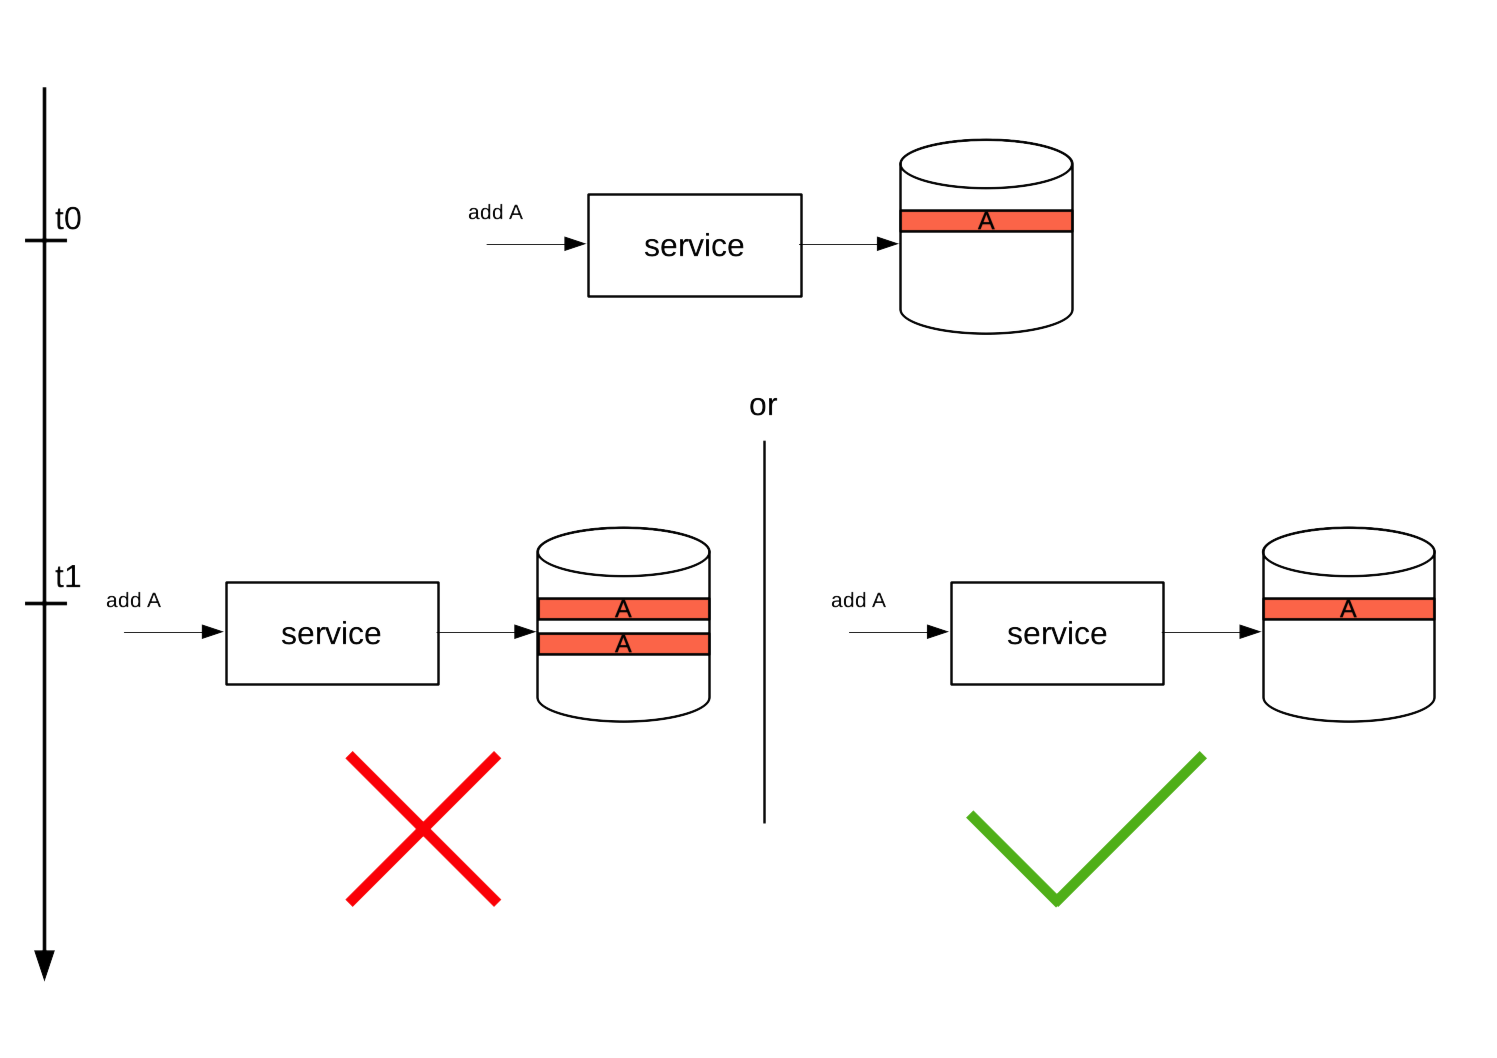
\includegraphics[height=6cm]{images/idempotence.png}}
	\end{frame}
	
	\begin{frame}
		\frametitle{Backward compatibility}
		\center{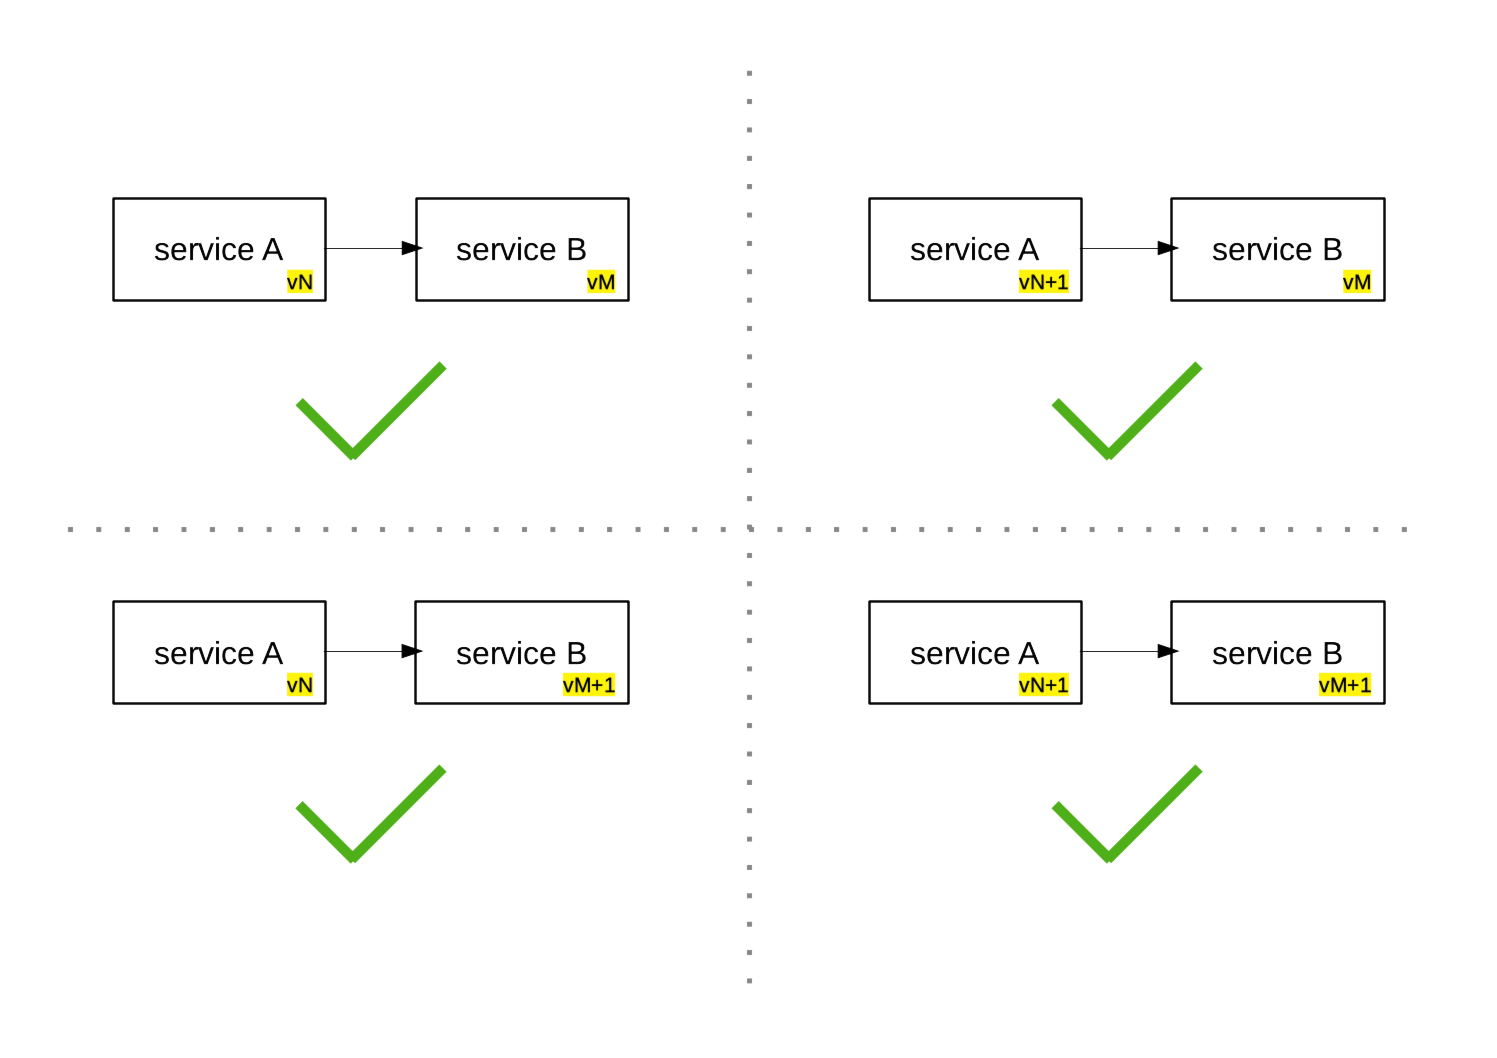
\includegraphics[height=6cm]{images/backwardCompatibility.png}}
	\end{frame}
	
	\begin{frame}
		\frametitle{Design for failure}
		
		\begin{center}
			\textit{Anything that can go wrong will go wrong.} [Murphy's law]
		\end{center}
		
		\visible<2->{\center{Be prepared!}}
	\end{frame}
		
	\section*{}
	
	\begin{frame}
		\center{Questions?}
	\end{frame}
	
\end{document}